\chapter{Representing distribution via Sigma-Points}


\section{Introduction}


\section{Factor operations}


\subsection{Dependencies: Transformations (QED)}

This is what sigma points were originally developed for and here they
can really shine. You simply get the sigma points for your input variable/vector
$X$, for each one of them apply the transformation to it to get the
corresponding sample in the space of $Y$, and from the combined set
of samples for $(X,Y)$, calculate a joint parametric representation
$p(X,Y)$. It is important though to match the type of distribution
of the joint to the properties of the transformation. For instance,
with $X$ a Gaussian, and $Y$ some monotonic transformation of it,
it probably makes sense to also use a Gaussian for the joint. If,
however, the transformation was non-monotonic, one should first determine
an appropriate target distribution type, possibly via laborious mathematical
derivation. For instance, if $Y=X^{2}$ the target distribution for
$Y$ should be Wishart/Gamma/Chi-squared, and the joint probably a
Gaussian-Wishart.


\subsection{Conditional Dependencies (QED)}

This one is a special case of the above mentioned transformations
-- the difference being that we now only know the transformation as
a distribution. If we have some prior distribution (including its
sigma points) for a parameter of the target density, we can predict
samples from the target density by means of each of these sigma points.
Maybe it is best to explain via an example.

\textbf{Example:} For instance, if we have a Gaussian prior for the
mean $\mu_{X}$ of a Gaussian RV $X$, the sigma points from $p(\mu_{x})$
are possible centroids around which samples of $X$ should be scattered.
But in contrast to the fixed transformations we encountered in the
previous section, we now will have a number of target samples associated
with each of the original sigma points. The original sigma-point weight
should now also be subdivided between these multiple target samples.
(This specific example with the prior mean we have just discussed
is the sigma-point version of linear Gaussian we have previously encountered.)

As was the case in the fixed transformations, it is important to match
the target distribution to the properties. For instance, it is not
fruitful to model the prior covariance of the target $X$ as a Gaussian
distribution in an effort to keep the full joint a Gaussian too. For
that case one will have to work with a Gaussian-Wishart / Gaussian-Inverse-Wishart
distribution.


\subsection{Product and division (Prefer parametric)}

Taking a Gaussian as an example, one can see that that product will
result in the precision matrices being summed. I.e. these operations
(amongst others) also affect the spread of the result. At the moment
I can see no easy way to directly determine the sigma points of the
result without first completing the operation in the parametric domain,
and from there calculating the new sigma points. Which is a long way
of saying that, at least at the moment, I dont know how to do these
operations with sigma points.


\subsection{Marginalisation (Conceptually easy, not expensive)}

This one is remarkably easy once you have the sigma points. You simply
knock the unwanted dimensions out of the sigma-points and recalculate
the parametric form from there. The hard work here then is in getting
the sigma points. On the other hand, once you have the right parametric
form to get to the sigma points, it probably is better to do the marginalisation
directly.


\subsection{Observation (Prefer parametric)}

At first I thought this also is an easy one to do. Your first calculate
a set of sigma points of the marginal that excludes the observed value.
Then you bump up the dimension by inserting the observed value into
the sigma points. But that is just plain wrong, the implied perpendicular
projection destroyed the information. Try it with a scalar Gaussian
and its mean and you'll see what I mean.

If I look at this from a Gaussian perspective, you are indeed projecting
on to the sub-space defined by your observation and the other free
variables. But it is not a perpendicular projection, it seems that
you are projecting in parallel with your $D-d$ principal axis, with
$D$ the original dimension and $d$ the number of observed variables.
But how does this generalise? Or, seeing that this happens outside
of the inference loop in any case, should we just do this in parametric
space? Will have to think about this a bit.


\subsection{Normalisation (Trivial)}

Nothing to be done here, the samples simply are. Normalisation takes
place automatically when they are converted to parametric form.


\subsection{Damping (Conceptually easy, but more expensive)}

I think this can be done easily by pooling the two reweighted sets
of sigma points and then recalculate the parametric form from that.
The expense here is in that the pooling doubled our set of sigma points.
To reduce them to the original number we will have to go parametric
and then recalculate them from there, which will be more expensive
than weak marginalisation.


\subsection{Distance measurement (Conceptually easy, and can be cheap)}

We need this for prioritising messages. And it seems quite normal
to the sigma-point domain. We have two sets of sigma-points and we
need to calculate the total distance between them. We can do this
at varying levels of complexity:
\begin{itemize}
\item measure the distance between the means. (Fast)
\item measure the distance of one set of sigma points to the mean of the
other and vice versa. (Easy enough)
\item measure the distance between corresponding points. Use something like
earth-mover's distance to define what 'corresponding' is. (More complex)
\end{itemize}
A possible complication is that distances are not comparible over
different sets of random variables. But I think that issue is also
part of the current implementation - to avoid that you will need some
information-theoretic criterion.


\section{Gaussians}


\subsection{Sigma-Point form }

From basic matrix algebra we have that $AA^{T}=\sum_{i}A_{i}A_{i}^{T},$
with $A_{i}$ the $i$'th column of $A$. This means that we can represent
the covariance matrix as:

\begin{align*}
\Sigma= & LL^{T}\\
= & \sum_{i=0}^{D-1}L_{i}L_{i}^{T},
\end{align*}


with $D$ the dimension and $L_{i}$ the $i$'th column of the lower
triangular Choleski matrix. However, we can also use a number of weighted
samples to find the sample covariance matrix as:

\begin{align*}
\hat{\Sigma}= & \frac{\sum_{i}w_{i}(\mathbf{x}_{i}-\mathbf{\mu})(\mathbf{x}_{i}-\mathbf{\mu}){}^{T}}{\sum_{i}w_{i}}
\end{align*}


Choosing $x_{i\pm}=\mathbf{\mu}\pm kL_{i}$, all with equal weighting
$w$, we have:

\begin{align*}
\hat{\Sigma} & =\frac{w\sum_{i=0}^{D-1}k^{2}L{}_{i}L{}_{i}{}^{T}+w\sum_{i=0}^{D-1}(-k)^{2}L{}_{i}L{}_{i}{}^{T}}{2Dw}\\
 & =\frac{2wk^{2}\sum_{i=0}^{D-1}L{}_{i}L{}_{i}{}^{T}}{2Dw}\\
 & =\frac{k^{2}\Sigma}{D}\\
 & =\Sigma,
\end{align*}


with $k=\sqrt{D}$. From this we deduce that if we place $2D$ equally
weighted samples symmetrically around the mean at positions $\mu\pm\sqrt{D}L_{i}$
we can retrieve the original mean and covariance from these samples,
i.e. they are an alternative parameterisation of the Gaussian. These
sample points are known as the sigma points.

The standard sigma point formulation also includes the mean as a sampling
point, in that case the other sigma points must move slightly further
away from the mean:

\begin{align}
x_0   &=\B{\mu}, && w_0 < 1 \text{ and} \\
x_{i\pm}&=\B{\mu}\pm\sqrt{\frac{D}{1-w_0}}L^{(i)},&&w_{i\pm}=\frac{1-w_0}{2D}&& i = 1\dots D. \label{eq:sigma-point}
\end{align}

The spacing of these samples are controlled by the centroid weight
$w_{0}<1$. Positive values move points further from mean, negative
values closer to the mean. If we choose $w_{0}=1-D$ all the sigma
points are spread one standard deviation away from the mean, irrespective
of their number. However, if we should group them differently (e.g.
via clustering) we run the risk of negative-definite covariances,
a definite no-no. The other weights are all equal and combined they
sum to one: $w_{j}=\frac{1-w_{0}}{2D},\,\, j\neq0$. Another popular
option is to have all sigma points equally weighted i.e. $w_{i}=\frac{1}{2D+1},\forall i=0:2D$
in which case the sigma points are spaced at $k=\sqrt{D+0.5}$. The
matrix square root $L$ can be found in any of a number of ways, Choleski
factorisation is a popular choice.


\paragraph{Example: }

Let us consider our earlier example:

\begin{align*}
\mathbf{\mu=} & \left[\begin{array}{r}
1\\
-3\\
4
\end{array}\right]\\
\Sigma= & \left[\begin{array}{rrr}
4 & 2 & -2\\
2 & 5 & -5\\
-2 & -5 & 8
\end{array}\right].
\end{align*}


Using Choleski decomposition it follows that:

\begin{align*}
L= & \left[\begin{array}{ccc}
2 & 0 & 0\\
1 & 2 & 0\\
-1 & -2 & 1.732
\end{array}\right].
\end{align*}


Using $w_{0}=\frac{0.5}{2D+1}=\frac{1}{14}$, i.e. $w_{i\neq0}=\frac{1+\frac{1}{4D}}{2D+1}=\frac{13}{84}$
we get the following seven displacement vectors:

\begin{tabular}{ccc}
 1.000000e+00 & -3.000000e+00 & 4.000000e+00   \\
 4.594868e+00 & -1.202566e+00 & 2.202566e+00   \\
 1.000000e+00 &  5.948681e-01 & 4.051319e-01   \\
 1.000000e+00 & -3.000000e+00 & 7.113247e+00   \\
-2.594868e+00 & -4.797434e+00 & 5.797434e+00   \\
 1.000000e+00 & -6.594868e+00 & 7.594868e+00   \\
 1.000000e+00 & -3.000000e+00 & 8.867529e-01
\end{tabular}

It is easy to verify that the weighted covariance estimate of these
is the same as the original covariance we started out with.

Note from Eq.~\ref{eq:sigma-point} that as $D$ increases, the sigma
points are being placed further and further from the mean. With fairly
low $D$ this might not seem to be a problem, but with for instance
$D=100$ all the sigma points occur at about 10 standard deviations
away. If we think of the sigma points as a carefully chosen sampling
of the original density, this means all the samples occur where we
would be extremely surprised to see any sample points at all! When
we want to reinterpret these sample points with for instance a clustering
algorithm, this will not do. All our samples are where none should
be, and none of our samples is where just about all of them should
be. We need to find a way to pull them back in closer to the origin.

One approach to this is the so-called Scaled Sigma-Point form. In
this approach we simply scale all our sigma points back with a scaling
factor $\alpha$ and then compensate for that when we do the covariance
estimate. But from a first cursory glance it seems that that will
only work when we keep these sample points in their original Gaussian,
but not if we were to for instance cluster them differently.

My pragmatic solution is to have three sets of sigma points, the first
a single one at the origin, then one set at $k=1$ and another at
$k=\sqrt{2D-0.5}$. The weighting of these points are all equal. Lets
check this out to see if it will work%
\footnote{Ok, I admit it. This did not come to me in a dream, it took a bit
of squigging. %
}:

Now we have 4D+1 sigma points, chosen as $x_{0}=\mathbf{\mu}$, $x_{i\pm}=\mathbf{\mu}\pm L_{i}$
and $x_{j\pm}=\mathbf{\mu}\pm\sqrt{2D-0.5}L_{j}$, all with equal
weighting $w$:

\begin{align*}
\hat{\Sigma} & =\frac{w\mathbf{00^{T}}+2w\sum_{i=0}^{D-1}L{}_{i}L{}_{i}{}^{T}+2w\sum_{i=0}^{D-1}(2D-0.5)L{}_{i}L{}_{i}{}^{T}}{w+2wD+2wD}\\
 & =\frac{\left(2w+2w(2D-0.5)\right)\sum L{}_{i}L{}_{i}{}^{T}}{w+4wD}\\
 & =\Sigma,
\end{align*}


The first $2D+1$ samples are located in the midst of the action.
Especially in higher-dimensional systems (i.e. $D\geq10$), however,
the last $2D$ samples are really only there to balance out the moments
by exerting influence from the far beyond no-mans-land.


\paragraph{Example: }

Using the same example as before we get the following sigma points:

\begin{tabular}{ccc}
 1.000000e+00 & -3.000000e+00 &  4.000000e+00\\
 3.000000e+00 & -2.000000e+00 &  3.000000e+00\\
 1.000000e+00 & -1.000000e+00 &  2.000000e+00\\
 1.000000e+00 & -3.000000e+00 &  5.732051e+00\\
-1.000000e+00 & -4.000000e+00 &  5.000000e+00\\
 1.000000e+00 & -5.000000e+00 &  6.000000e+00\\
 1.000000e+00 & -3.000000e+00 &  2.267949e+00\\
 5.690416e+00 & -6.547921e-01 &  1.654792e+00\\
 1.000000e+00 &  1.690416e+00 & -6.904158e-01\\
 1.000000e+00 & -3.000000e+00 &  8.062019e+00\\
-3.690416e+00 & -5.345208e+00 &  6.345208e+00\\
 1.000000e+00 & -7.690416e+00 &  8.690416e+00\\
 1.000000e+00 & -3.000000e+00 & -6.201920e-02

\end{tabular}


\subsection{The model\label{sec:sigma_point_model}}

We are going to assume that $\mathbf{Y}=\text{f}(\mathbf{X})+\text{{noise}}$,
with $\mathbf{X}$ a multi-dimensional Gaussian RV, $\text{f}$ a
generic non-linear function that transforms $\mathbf{X}$ into another
(probably non-Gaussian) vector, and the noise zero-mean with covariance
$\Sigma_{NN}$. We are going to approximate the joint $(\mathbf{X},\mathbf{Y})$
as being jointly Gaussian. For this, in addition to the already available
$\mathbf{\mu_{X}}$ and $\Sigma_{\mathbf{XX}}$ we will also need
$\mathbf{\mu_{Y}}$, $\Sigma_{\mathbf{XY}}$ and $\Sigma_{\mathbf{YY}}$.
Assuming that we can use $\text{f}$ to map the sigma points of $\mathbf{X}$
to a noiseless version of $\mathbf{Y}$, we can now determine expressions
for these quantities.

The mean isn't rocket science:

\begin{align}
\mathbf{\mu_{Y}} & =\frac{1}{N}\sum_{n}\mathbf{y}_{n}.
\end{align}


Calculating the cross-covariance term (in the absence of noise):

\begin{align}
\Sigma_{\mathbf{XY}}= & \mathbb{E}[(\mathbf{X}-\mathbb{E}[\mathbf{X}])(\mathbf{Y}-\mathbb{E}[\mathbf{Y}])^{T}\nonumber \\
= & \mathbb{E}\left[\mathbf{X}\mathbf{Y}^{T}-\mathbf{X}\mathbb{E}[\mathbf{Y}]^{T}-\mathbb{E}[\mathbf{X}]\mathbf{Y}^{T}+\mathbb{E}[\mathbf{X}]\mathbb{E}[\mathbf{Y}]^{T}\right]\nonumber \\
= & \mathbb{E}\left[\mathbf{X}\mathbf{Y}^{T}-\mathbf{X}(\frac{1}{N}\sum_{n}\mathbf{y}_{n})^{T}-(\frac{1}{N}\sum_{n}\mathbf{x}_{n})\mathbf{Y}^{T}+(\frac{1}{N}\sum_{n}\mathbf{x}_{n})(\frac{1}{N}\sum_{n}\mathbf{y}_{n})^{T}\right]\nonumber \\
= & \frac{1}{N}\sum_{m}\left[\mathbf{x}_{m}\mathbf{y}_{m}^{T}-\mathbf{x}_{m}(\frac{1}{N}\sum_{n}\mathbf{y}_{n})^{T}-(\frac{1}{N}\sum_{n}\mathbf{x}_{n})\mathbf{y}_{m}^{T}+(\frac{1}{N}\sum_{n}\mathbf{x}_{n})(\frac{1}{N}\sum_{n}\mathbf{y}_{n})^{T}\right]\nonumber \\
= & \frac{1}{N}\sum_{m}\mathbf{x}_{m}\mathbf{y}_{m}^{T}-\frac{1}{N}\sum_{m}\mathbf{x}_{m}(\frac{1}{N}\sum_{n}\mathbf{y}_{n})^{T}-\frac{1}{N}\sum_{m}(\frac{1}{N}\sum_{n}\mathbf{x}_{n})\mathbf{y}_{m}^{T}+\frac{1}{N}\sum_{m}(\frac{1}{N}\sum_{n}\mathbf{x}_{n})(\frac{1}{N}\sum_{n}\mathbf{y}_{n})^{T}\nonumber \\
= & \frac{1}{N}\sum_{m}\mathbf{x}_{m}\mathbf{y}_{m}^{T}-(\frac{1}{N}\sum_{m}\mathbf{x}_{m})(\frac{1}{N}\sum_{n}\mathbf{y}_{n})^{T}-(\frac{1}{N}\sum_{n}\mathbf{x}_{n})(\frac{1}{N}\sum_{m}\mathbf{y}_{m})^{T}+(\frac{1}{N}\sum_{n}\mathbf{x}_{n})(\frac{1}{N}\sum_{n}\mathbf{y}_{n})^{T}\nonumber \\
= & \frac{1}{N}\sum_{m}\mathbf{x}_{m}\mathbf{y}_{m}^{T}-\frac{1}{N}\sum_{m}\mathbf{x}_{m}\frac{1}{N}(\sum_{n}\mathbf{y}_{n})^{T}\nonumber \\
= & \frac{1}{N}\sum_{m}(\mathbf{x}_{m}\mathbf{y}_{m}^{T})-\mathbf{\mu_{x}}\mathbf{\mu_{y}}^{T}.
\end{align}


The measurement noise should not influence this cross-covariance since
it is zero mean and only enters the equation linearly via $\mathbf{Y}=\mathbf{Y}_{{noiseless}}+\epsilon$.

Similarly the covariance term for $\mathbf{Y}$ is determined (in
the absence of noise) as:

\begin{align}
\Sigma_{\mathbf{YY}}= & \frac{1}{N}\sum_{m}(\mathbf{y}_{m}\mathbf{y}_{m}^{T})-\mathbf{\mu_{y}}\mathbf{\mu_{y}}^{T}.
\end{align}


To incorporate the measurement noise we simply add $\Sigma_{NN}$
to the above.


\subsection{Modelling linear projections $\mathbf{Y}=A\mathbf{X}$ via sigma
points}

The case where $A$ is a known matrix, was already covered in the
chapter on linear Gaussians. However, when $A$ is a random matrix,
we need more extensive machinery, which happens to also cover the
linear Gaussians as a special case.


\subsection{Gaussian priors approximated (again) as Gaussians}

It is usual to model the mean and covariance of a multidimensional
Gaussian by means of the Gauss-Wishart distribution. In this section
we are going to explore another avenue that makes exclusively use
of Gaussians. Whether this will prove practically useful I currently
do not know, therefore for the while being it might be best to just
consider this as mental meandering. In the following we will consider
the Gaussian parameters $\mathbf{\mu}$ and $\Sigma$ of a $D$-dimensional
Gaussian RV $\mathbf{X}$.


\subsubsection{Known $\Sigma$, unknown $\mathbf{\mu}$}

The most direct approach here is to model this situation with a linear
Gaussian -- $p(\mathbf{\mu})$ is our prior distribution, the projection
matrix is $I_{D}$ and our measurement noise is $\Sigma$. However,
in the following we instead explore achieving the same result by making
use of sigma points.

We need some initial distribution for $\mathbf{\mu}$, typically $\mathcal{N}(0_{D},\sigma^{2}I_{D})$
(but of course it is also trivial to specify the variances individually).
For each of the $2D+1$ sigma points of $\mathbf{\mu}$, combine its
$2D+1$ sigma points spread around it according to the covariance
$\Sigma$. This gives a total of $(2D+1)^{2}$ sigma-points, each
being a $D$-dimensional sample of $\mathbf{X}$. Combined with the
original $D$-dimensional $\mathbf{\mu}$ we therefore have a $2D$-dimensional
joint $p(\mathbf{X},\mathbf{\mu})$ (as is described in section \ref{sec:sigma_point_model}).


See Figure~\ref{fig:bayesmeanest2d} for an example utilising this.

\begin{figure}
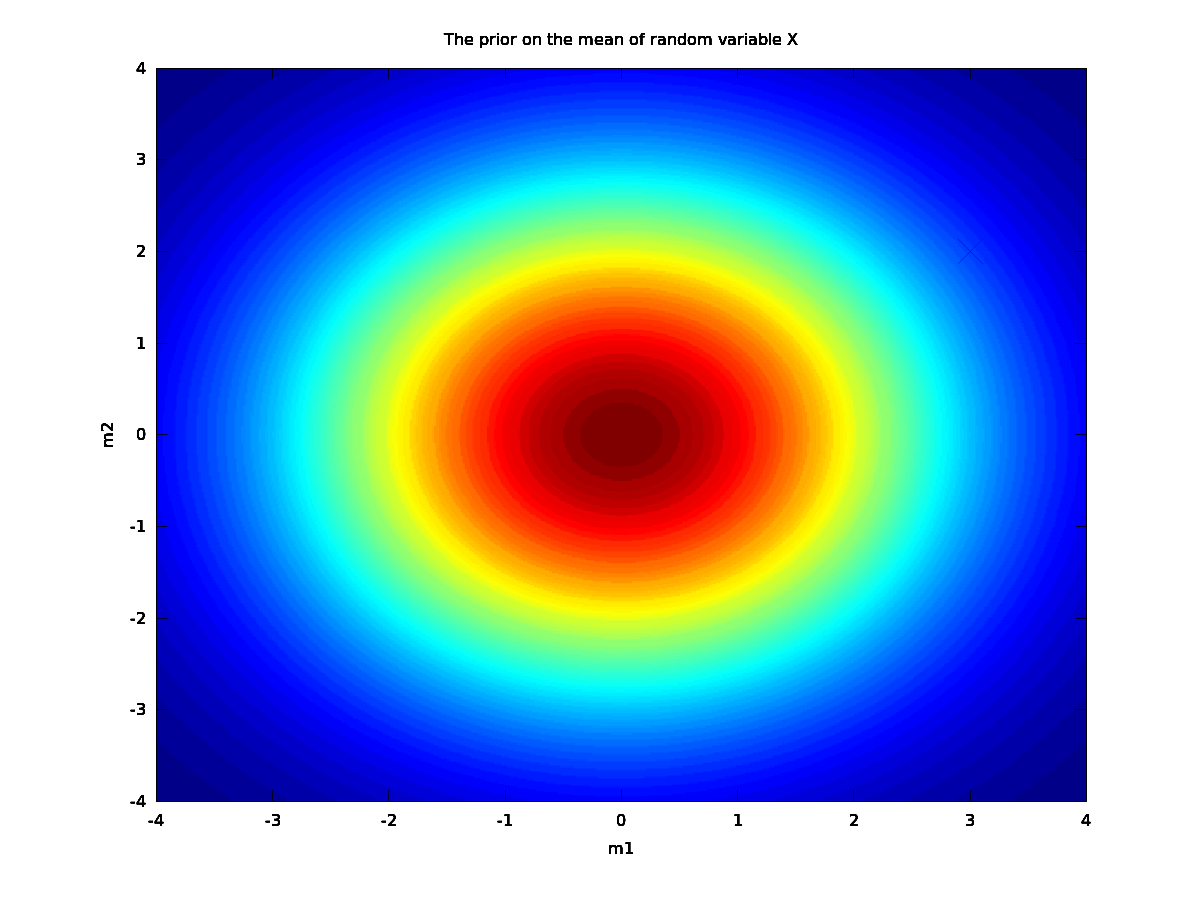
\includegraphics[width=7cm]{prior_of_mean}\\
The prior $p(\mu)$.
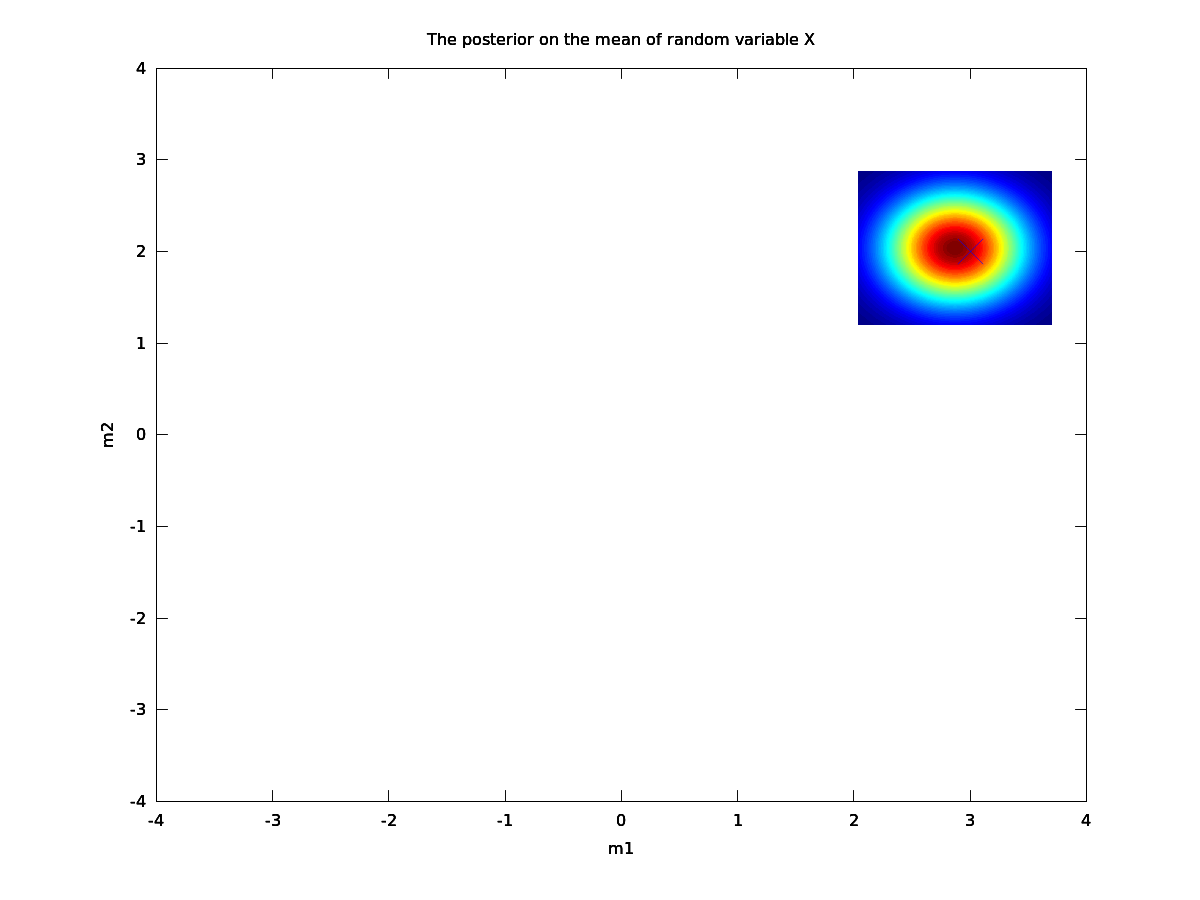
\includegraphics[width=7cm]{posterior_of_mean}\\
The posterior estimate $p(\mu|\mathbf{X}_{1\ldots33})$ (i.e. after
33 observations).
\caption{Bayesian estimation of the mean $\mu$ of RV $\mathbf{x}$ given that
we know the covariance $\Sigma$. The actual position of the mean
is at (3,2) and is marked with a (rather faint) 'X'. The important
point here is not so much that after observing $\mathbf{X}_{1\ldots33}$
the estimate of the mean is pretty close (ML estimation will also
give that), but that the uncertainty about the estimate is also quantified.
Subtly beautiful!}
\label{fig:bayesmeanest2d}
\end{figure}



\subsubsection{Known $\mathbf{\mu}$, unknown $\Sigma$}

\textbf{Dont bother, this does not work.} $\Sigma$ remains uncorrelated
with both $\mathbf{\mu}$ and $\mathbf{X}$, so we can not infer anything
about it. It seems that we will have to bite the bullet and add a
NIW (Normal Inverse Wishart) to EMDW.

Here the linear Gaussian approach will fail us, the model is inherently
non-linear and the conjugate priors no longer are Gaussian (either
gamma or Wishart). However, in the following we will make use of sigma
points to model the result of this non-linear operation once again
with a Gaussian.

Because of symmetry there is $\frac{D(D+1)}{2}$ components we need
to model in $\mathbf{\Sigma}$. It makes sense to model the variances
(on the diagonal) differently from the covariances (off-diagonal)
-- we briefly postpone the discussion of the details of this to the
next paragraph. Assuming that we have a $\frac{D(D+1)}{2}$-dimensional
Gaussian density available for these components, we can proceed to
find its $2\frac{D(D+1)}{2}+1=D^{2}+D+1$ sigma points. Each of these
sigma points represents a different covariance matrix, and this covariance
matrix describes the spread around the known $D$-dimensional mean
vector $\mathbf{\mu}$. Each such combination can thus be represented
by $2D+1$ sigma points giving a total of $(2D+1)(D^{2}+D+1)=2D^{3}+2D^{2}+3D+1$
sigma points, each being a $D$-dimensional sample of $\mathbf{X}$.
Combined with the original $\frac{D(D+1)}{2}$-dimensional $\Sigma$
we therefore have a $\frac{D^{2}+3D}{2}$-dimensional joint $p(\mathbf{X},\Sigma)$.

We now return to the topic of how exactly to model the prior on the
covariances: Because we are modelling a covariance matrix which is
supposed to be positive definite, with a Gaussian which implicitly
has infinite (and thus also negative) support, we are running a severe
risk of running into trouble. Indeed, at this moment I still am unsure
if the procedure I am about to describe is adequate to save our butts,
but lets give it a shot.

It seems that the safest place to start is the correlation coefficient
version of the desired covariance matrix (see \ref{par:corr_coef_form}).
In this normalized version all variances are unity, and the magnitude
of all covariances should be strictly less than one (and even then
we are still not guaranteed that the matrix as a whole is positive
definite).
\begin{itemize}
\item If we now represent these normalised variances $\rho_{ii}$ with Gaussians
with a mean value
\begin{equation}
\mu_{\rho_{ii}}=1,
\end{equation}
 we should try to keep their standard deviations $\sigma_{\rho_{ii}}$small
enough to make negative values of $\rho_{ii}$ very unlikely. Since
samples exceeding about three standard deviations away from the mean
should be rare, this seems to imply that we should choose these standard
deviations at about $\sigma_{\rho_{ii}}=\frac{1}{4}$. But we should
also remember that we are going to represent them via sigma points
which, at least in the standard version we use here, are placed at
about $\sqrt{D+0.5}$ standard deviations away from the mean and this
also should still be positive. Therefore we have
\begin{equation}
\sigma_{\rho_{ii}}\leq\text{min}(\frac{1}{4},\frac{1}{\sqrt{D+0.5}}).
\end{equation}

\item For the off-diagonal correlation coefficients we know that $-1<\rho_{ij}<1$.
Therefore a mean
\begin{equation}
\mu_{\rho_{ij}}=0,
\end{equation}
and standard deviations
\begin{equation}
\sigma_{\rho_{ij}}\leq\text{min}(\frac{1}{4},\frac{1}{\sqrt{\frac{D(D-1)}{2}+0.5}})
\end{equation}
 seems appropriate.
\item As a final step we now need to rescale to the actual non-normalised
variances we want to use. For the normalised version we currently
have:
\[
\mathbf{\rho}\sim\mathcal{N}\left(\left[\begin{array}{c}
\mathbf{1}_{D}\\
\mathbf{0}_{\frac{D(D-1)}{2}}
\end{array}\right],\left[\begin{array}{cc}
\sigma_{\rho_{ii}}^{2}I_{D} & \mathbf{0}\\
\mathbf{0} & \sigma_{\rho_{ij}}^{2}I_{\frac{D(D-1)}{2}}
\end{array}\right]\right).
\]
Assuming that we actually wanted variances $\sigma_{i}^{2}$ as the
expected value of the diagonal elements of $\mathbf{X}$'s covariance
matrix $\Sigma,$ we simply rescale to $\mathbf{\gamma}_{ii}=\sigma_{i}^{2}\mathbf{\rho}_{ii}$
to get:
\begin{equation}
\mathbf{\gamma}\sim\mathcal{N}\left(\left[\begin{array}{c}
\sigma_{1}^{2}\\
\vdots\\
\sigma_{D}^{2}\\
0_{1}\\
\vdots\\
0_{\frac{D(D-1)}{2}}
\end{array}\right],\left[\begin{array}{cccccc}
\sigma_{1}^{4}\sigma_{\rho_{ii}}^{2} & 0 & \hdots & \hdots & \hdots & 0\\
0 & \ddots & \ddots & \ddots & \ddots & \vdots\\
\vdots & \ddots & \sigma_{D}^{4}\sigma_{\rho_{ii}}^{2} & \ddots & \ddots & \vdots\\
\vdots & \ddots & \ddots & \sigma_{1}^{2}\sigma_{2}^{2}\sigma_{\rho_{ij}}^{2} & \ddots & \vdots\\
\vdots & \ddots & \ddots & \ddots & \ddots & 0\\
0 & \hdots & \hdots & \hdots & 0 & \sigma_{(D-1)}^{2}\sigma_{D}^{2}\sigma_{\rho_{ij}}^{2}
\end{array}\right]\right).
\end{equation}



For the istropic case we, of course, simply replace $\sigma_{i}^{2}=\sigma^{2}$.

\end{itemize}

\subsubsection{Both $\mathbf{\mu}$ and $\Sigma$ unknown}

\textbf{Dont bother, this does not work.} $\Sigma$ remains uncorrelated
with both $\mathbf{\mu}$ and $\mathbf{X}$, so we can not infer anything
about it. It seems that we will have to bite the bullet and add a
NIW (Normal Inverse Wishart) to EMDW.

Now things are doubly non-linear -- firstly due to $\Sigma$ being
quadratic, and secondly because we are combining two different sets
of random variables ($\mathbf{\mu}$ and $\Sigma$) into the estimate
densities in the estimate of a third ($\mathbf{X}$). Only do this
if you have non-trivial estimates available for both $\mathbf{\mu}$
and $\Sigma$, otherwise you are very likely to end up with a diagonal
covariance matrix for the final joint, making everything independent.
Not very helpful.

We use the same machinery we implemented for the known $\mathbf{\mu}$,
unknown $\Sigma$ case, but now repeated for each of the $2D+1$ sigma
points of $\mathbf{\mu}$. This gives us an impressive grand total
of $(2D+1)(2D^{3}+2D^{2}+3D+1)$ sigma points and the dimension of
the joint $p(\mathbf{X},\mathbf{\mu},\Sigma)$ is $\frac{D^{2}+5D}{2}$.
